% =====================================================================
%  Capitolo 7 — Eventi, nodi e variabili: la prima lezione di
%  programmazione con i Blueprint di Unreal Engine (Game Design, primo
%  anno)
%  Fonte: trascrizione della lezione GD7 (Game Design, primo anno),
%  lezione ibrida (in aula e da remoto, su Zoom e Discord).
%  Contenuti, nell'ordine della lezione: presentazioni; C++ e Blueprint;
%  i tre concetti (eventi, nodi, variabili); il progetto in terza
%  persona; il primo Blueprint (Actor "test" con un cubo); Begin Play,
%  Event Tick e Print String; le variabili, i loro tipi e i loro colori;
%  GET e SET; il contatore che sale a ogni frame; gli eventi da
%  tastiera, Launch Character, Set Actor Scale 3D, Set Actor Location;
%  il Character Movement (Jump Z Velocity, Max Walk Speed); Delay e
%  Branch; la trigger box (Box Collision, On Component Begin Overlap,
%  Cast To ThirdPersonCharacter, il Target); Spawn Actor, Simulate
%  Physics, Destroy Actor; le monete e il contatore sul personaggio;
%  la lingua dell'editor; Open Level, Play Sound 2D, Quit Game; il task
%  in classe dei due livelli; le monete che ruotano; l'Event Tick e i
%  delta seconds; il ripasso della trigger box; il sistema di vita;
%  Actor, Pawn e Character; Line Trace By Channel; le regole dei
%  collegamenti; le domande di Federica (il filo bianco, i colori, il
%  Delay, l'interfaccia); il riepilogo del task; la chiusura.
%  Integrazioni dal libro "Blueprints Visual Scripting for Unreal
%  Engine 5" (Romero, Sewell), segnalate come approfondimenti.
%
%  Pacchetti richiesti nel preambolo del libro (già presenti nel
%  main.tex): \usepackage{booktabs}, \usepackage{amsmath},
%  \usepackage{tikz} con
%    \usetikzlibrary{shapes.geometric,shapes.symbols,shapes.misc,
%      arrows.meta,positioning,calc,fit}
%  (le librerie vanno caricate nel preambolo, non nel capitolo).
%  Tutte le etichette di questo capitolo hanno il prefisso "gd7:"
%  (gd7:sec:..., gd7:fig:..., gd7:tab:...) e tutti gli stili TikZ il
%  prefisso "gd7" (gd7node, gd7exec, ...), per non collidere con gli
%  altri capitoli.
%
%  Nota sulla fonte: la trascrizione automatica è in questo caso
%  particolarmente rovinata. La lezione è quasi tutta pratica (il
%  docente gira tra i banchi e guarda gli schermi condivisi), e i lunghi
%  tratti di lavoro individuale sono stati trascritti come frasi senza
%  senso o ripetute in loop, a volte con interi brani captati da una
%  fonte esterna (una radio o un video: frasi sul "mercato del lavoro",
%  sul "Parlamento", sugli "egiziani"), che qui sono ovviamente omessi.
%  Diversi nomi di nodi e di giochi sono storpiati: dove il riferimento è
%  ricostruibile con certezza lo si riporta nella forma corretta; dove
%  non lo è, lo si segnala in nota invece di indovinare. Le figure sono
%  ricostruzioni schematiche dei grafi costruiti a lezione, non
%  screenshot.
% =====================================================================

\chapter[Eventi, nodi e variabili]{Eventi, nodi e variabili: la prima
lezione di programmazione con i Blueprint}
\label{gd7:cap:blueprint}

Fino a questo punto il corso di Game Design ha lavorato quasi solo su carta:
che cos'è un gioco, come si produce, come si documenta, come si passa da un
problema a un'idea e da un'idea a un flowchart (capitoli
\ref{cap:introduzione-game-design}--\ref{cap:brainstorming-flowchart}). Con
questo settimo capitolo si cambia completamente registro: si apre
\textbf{Unreal Engine} e si comincia a \textbf{programmare}, con i
\textbf{Blueprint}. Il flowchart del capitolo precedente, del resto, era già
una mezza introduzione: un Blueprint è, a guardarlo, un flowchart che il
computer esegue.

Il docente lo dice subito, e lo ripeterà più volte durante la giornata: la
lezione di oggi è ``\textbf{super importante}'', perché ``quello che faremo
qui oggi si baserà su tutto quanto il resto dei prossimi \textbf{tre anni} di
programmazione''. Per questo chiede alla classe di fermarlo a ogni dubbio,
anche il più piccolo. Chi ha già seguito il corso breve su Unreal
(capitoli~\ref{ue1:cap:intro} e~\ref{ue2:cap:blueprint}) troverà qui molti
concetti noti, ma visti da un'altra angolazione e con un altro obiettivo: non
costruire un piccolo gioco guidato passo per passo, ma \textbf{prendere la
mano} con i tre mattoni su cui si regge tutto il resto.

La lezione è \textbf{ibrida}: una parte della classe è in aula, una parte
(Valerio, Federica, Mattia) è collegata da remoto su Zoom e condivide lo
schermo su Discord. Il computer del docente, purtroppo, non regge: crasha più
volte, va ``lentissimo'', e a un certo punto rende impossibile guardare gli
schermi condivisi (``cambieremo PC a breve, non vi preoccupate''). La
struttura della lezione, e quindi del capitolo, è questa:
\begin{enumerate}
  \item le \textbf{presentazioni} e il quadro generale: C++ e Blueprint, e i
        \textbf{tre concetti} che bisogna imparare davvero
        (sezioni~\ref{gd7:sec:presentazioni} e~\ref{gd7:sec:tre-concetti});
  \item il progetto in terza persona e il \textbf{primo Blueprint}, un
        semplice cubo (sezioni~\ref{gd7:sec:progetto}
        e~\ref{gd7:sec:primo-blueprint});
  \item gli \textbf{eventi} (Begin Play, Event Tick) e il primo nodo, il
        Print String (sezione~\ref{gd7:sec:eventi});
  \item le \textbf{variabili}: i tipi, i colori, il GET e il SET, il
        contatore che sale a ogni \emph{frame}
        (sezioni~\ref{gd7:sec:variabili} e~\ref{gd7:sec:get-set});
  \item il \textbf{personaggio}: gli eventi da tastiera, il lancio, la
        scala, il teletrasporto e il \textbf{Character Movement}
        (sezioni~\ref{gd7:sec:personaggio} e~\ref{gd7:sec:movement});
  \item le \textbf{interazioni tra oggetti}: la trigger box, il
        \emph{cast}, il \emph{target}, lo \emph{spawn}, la fisica
        (sezioni~\ref{gd7:sec:trigger} e~\ref{gd7:sec:spawn});
  \item le \textbf{monete} e il contatore sul personaggio
        (sezione~\ref{gd7:sec:monete});
  \item altri nodi utili e il \textbf{task in classe}: due livelli e almeno
        una zona che cambia il personaggio
        (sezioni~\ref{gd7:sec:altri-nodi} e~\ref{gd7:sec:task});
  \item l'Event Tick e i \textbf{delta seconds}
        (sezione~\ref{gd7:sec:delta});
  \item il ripasso, il \textbf{sistema di vita}, Actor, Pawn e Character, il
        Line Trace (sezioni~\ref{gd7:sec:ripasso}--\ref{gd7:sec:classi});
  \item le \textbf{regole dei collegamenti} e le domande di chi parte da
        zero: che cos'è il filo bianco, che cosa vogliono dire i colori
        (sezioni~\ref{gd7:sec:regole} e~\ref{gd7:sec:federica}).
\end{enumerate}

% ---------------------------------------------------------------------
\section{Prima di cominciare: chi c'è, e chi ha già programmato}
\label{gd7:sec:presentazioni}

\subsection{Le versioni dell'engine}

Mentre si aspetta che arrivino tutti (``aspettiamo ancora cinque minuti''),
la prima domanda è sulla versione di Unreal scaricata: la 5.6, la 5.7, la
5.8? Qualcuno ha già scaricato la 5.8. Per il docente non fa differenza:
``tanto è uguale, non vi cambia molto''. Lo ribadirà più tardi a uno studente
che sta reinstallando l'engine: meglio avere la stessa versione degli altri
(la 5.8), ma ``se sei sulle ultime versioni non ti cambierà praticamente
nulla''; anche una 5.4 ``non è un problema''. Per le cose che si fanno oggi
le differenze tra le versioni recenti sono irrilevanti.

\subsection{Un giro di presentazioni}

Mancando ancora un paio di minuti, il docente chiede a ciascuno di
raccontare qualcosa di sé: che cosa fa, che cosa gli piace, \textbf{se ha mai
programmato} oppure no. Il quadro che ne esce è quello tipico di un primo
anno, e vale la pena riportarlo perché spiega il ritmo della lezione:
\begin{itemize}
  \item chi viene dal liceo scientifico ha visto un po' di \textbf{C},
        \textbf{Python} e un po' di \textbf{SQL}: ``comunque già un po' di
        basi'';
  \item chi viene da altri indirizzi, come Francesco, che ha fatto il
        \textbf{classico}, parte ``da zero zero zero zero'';
  \item Valerio è un \textbf{grafico}: zero assoluto, se non un po' di
        codice per il web, ``molto, molto poco'';
  \item Mattia (Maestri) arriva da un'altra accademia di videogiochi, quella
        di Bologna, dove era al secondo anno: ha già usato Unreal ``anche se
        per poco'', con i Blueprint ``a un livello basico'', e si muove già
        un po' nell'editor, ma è ``una materia in cui faccio abbastanza
        fatica'';
  \item Federica dichiara una conoscenza ``pari a zero, anche meno''
        (``tranquilla, non sei l'unica qui'').
\end{itemize}

\paragraph{I giochi preferiti.} Il giro comprende anche i giochi preferiti.
Tra quelli che la trascrizione restituisce in modo riconoscibile: un gruppo di
giochi ``un pochettino cupi'', tra cui \emph{The Binding of Isaac}; la saga di
\emph{Monster Hunter} per Mattia; \emph{Yakuza 0} e \emph{Dave the Diver}
(``bellissimo'') per Valeria; e per Federica e Daniele due titoli ``molto
indie''.\footnote{Diversi titoli sono irriconoscibili nella trascrizione
automatica (``It's All World'', ``il signor Sky'', ``Otherwise'',
``Discollision''); non li si ricostruisce per non attribuire agli studenti
giochi che non hanno nominato.} Il docente non li conosce tutti e lo ammette
senza problemi (``non lo conosco, colpa mia''): il punto del giro non è il
quiz, è sapere \textbf{da dove parte} ciascuno.

\paragraph{Chi parte da zero.} Più avanti, a lezione inoltrata, Federica dirà
di essersi persa all'inizio per colpa dei crash e di due computer in due
stanze diverse. La risposta del docente fissa il tono di tutto il corso:
``siamo alla prima lezione, non puoi essere indietro. Non è possibile stare
indietro, proprio matematicamente.'' Se serve rifarla da capo, la si rifà da
capo. L'importante è non restare indietro \emph{dopo}: ``se avete dubbi me li
dovete fare qua, adesso, non dopo''. Per tutto il resto c'è Discord, dove si
può scrivere al docente (e, se è grave, chiedere una chiamata).

% ---------------------------------------------------------------------
\section{Due modi di programmare, tre concetti da imparare}
\label{gd7:sec:tre-concetti}

\subsection{C++ e Blueprint}

Unreal è un \textbf{engine}, uno strumento per fare giochi. Lo si può
programmare in due modi:
\begin{itemize}
  \item in \textbf{C++}, il linguaggio scritto ``classico''. Nel corso non lo
        si vedrà, ``se non proprio una cosina microscopica al secondo
        anno'';
  \item con i \textbf{Blueprint}, che saranno lo strumento di tutto il
        corso. I due sistemi, in realtà, ``parlano tra loro'', ma questo per
        ora non importa.
\end{itemize}
La comodità dei Blueprint è che non sono codice scritto come lo vedono i
programmatori: sono composti da \textbf{blocchetti colorati}, e ``componendo
quelli fate tutto''. Non serve ricordarsi come si scrive un comando né dove va
una virgola: si fa tasto destro e si cerca.

\subsection{Eventi, nodi, variabili}

Il cuore della lezione sta in una frase: i Blueprint sono composti
\textbf{soltanto da tre cose}, ``le uniche tre che dovete imparare
veramente''.
\begin{description}
  \item[I nodi] sono \textbf{tutto ciò che si può fare}: stampare una
        scritta, lanciare il personaggio, spostare un oggetto, distruggerlo.
  \item[Le variabili] sono \textbf{le cose che cambiano}: le informazioni che
        il gioco legge e modifica (quante monete ho, quanto salto in alto,
        dove mi trovo).
  \item[Gli eventi] sono \textbf{l'inizio del codice}: il momento in cui
        qualcosa comincia a succedere (l'oggetto viene creato, passa un
        \emph{frame}, il giocatore preme un tasto, qualcosa entra in
        un'area).
\end{description}
``Basta, non è che c'è altro.'' Se si capiscono bene questi tre concetti,
``siamo a posto, perché tutto quello che arriverà dopo si basa su quello''.
Il docente invita a scriverseli.

\paragraph{Approfondimento: il percorso di esecuzione.} Romero e Sewell, nel
secondo capitolo del loro libro sui Blueprint, danno un nome preciso a quello
che a lezione si vede con le mani: l'esecuzione di un Blueprint
\textbf{comincia da un nodo evento} (rosso) e poi \textbf{segue il filo
bianco da sinistra a destra} fino all'ultimo nodo. Questo filo si chiama
\emph{execution path}, il percorso di esecuzione; i pin bianchi dei nodi sono
i \emph{pin di esecuzione}, quelli colorati i \emph{pin dei dati}. È la stessa
distinzione che il docente spiegherà a fine lezione con l'immagine della
corrente elettrica (sezione~\ref{gd7:sec:federica}).

% ---------------------------------------------------------------------
\section{Il progetto in terza persona}
\label{gd7:sec:progetto}

\subsection{Creare il progetto}

Si apre Unreal, nella versione che si ha, e si crea un \textbf{progetto nuovo
da zero} con il template \textbf{Third Person} (la categoria è quella dei
giochi, \emph{Games}, poi \emph{Third Person}), lasciando tutto il resto
``esattamente così com'è''. Il nome proposto è \textbf{GG1} seguito dalla
data. Il template in terza persona ha un vantaggio: c'è già un
\textbf{personaggio di base} che si può controllare, quello standard.

\paragraph{Se il template è sbagliato.} Un paio di studenti si ritrovano con
una mappa diversa da quella del docente (``tipo un'arena, con le strutture
verdi''): hanno scelto una variante sbagliata. Le soluzioni sono due:
ricreare il progetto, oppure, se il progetto è vuoto, usare \textbf{Add
Feature} (aggiungi funzionalità), scegliere il pacchetto in terza persona e
fare \emph{Add}: ``così torni esattamente dove siamo''.

\subsection{L'editor, in due parole}

Una volta caricato (``spero che il computer regga''), l'editor si presenta con
due zone principali:
\begin{itemize}
  \item la \textbf{viewport}, ``dove c'è tutto quanto ciò che vediamo nella
        scena''. Premendo \textbf{Play} parte il gioco (``incredibile''), e
        ci si muove come in un normale gioco in terza persona;
  \item il \textbf{Content Browser}, qua sotto, con gli \textbf{asset}:
        ``praticamente tutto ciò che ci sarà nel nostro gioco'', il codice,
        le texture, le mesh, i suoni, organizzati in cartelle. ``Molto, molto
        facile.''
\end{itemize}

\subsection{Il personaggio: viewport ed Event Graph}

Nel Content Browser, nella cartella \emph{ThirdPerson} $\rightarrow$
\emph{Blueprints}, si trova il \textbf{ThirdPersonCharacter}, il personaggio
che compare quando si preme Play. Aprendolo si vedono molte schermate e molti
tasti, ma il docente rassicura: ``non fatevi intimorire''. La cosa importante
è che un Blueprint è suddiviso, fondamentalmente, in due parti:
\begin{itemize}
  \item la \textbf{viewport}, la parte \textbf{visiva} dell'oggetto;
  \item l'\textbf{Event Graph}, la parte del \textbf{codice}.
\end{itemize}
Per semplificarsi ancora di più la vita, però, il docente lo chiude subito:
si parte da zero, con un oggetto nuovo su cui mettere il codice.

% ---------------------------------------------------------------------
\section{Il primo Blueprint: un cubo}
\label{gd7:sec:primo-blueprint}

\subsection{Blueprint Class, Actor}

Nel Content Browser, in uno spazio vuoto della cartella \emph{Content}: tasto
destro, \textbf{Blueprint Class}. È il comando per creare un \textbf{oggetto
nuovo qualsiasi}: ``potrebbe essere un personaggio, una macchina, il gatto che
passa, un muro, qualsiasi cosa che si mette nella scena''. La finestra che si
apre offre molte opzioni, che per ora si ignorano completamente: si sceglie
sempre la prima, \textbf{Actor}, ``che è la cosa base''. Il docente lo chiama
\textbf{test}, ``per rimanere sul semplice''. Doppio clic, e il Blueprint si
apre. (La differenza tra Actor, Pawn e Character arriverà verso la fine della
lezione, sezione~\ref{gd7:sec:classi}.)

\subsection{Un oggetto visibile, e più volte in scena}

L'oggetto appena creato, visivamente, è il vuoto: non c'è niente. Per
identificarlo gli si mette un \textbf{cubo}: \textbf{Add}, \emph{Cube}. ``Così
ora questo oggetto è effettivamente un cubo.'' Non ha ancora codice, ma lo si
può già \textbf{trascinare nella scena}, e lo si può fare \textbf{più volte}:
ogni copia trascinata è un elemento in scena. Il docente ne piazza tre; premendo
Play, i tre cubi sono lì. ``Roba facilissima.''

\paragraph{Approfondimento: classe e istanza.} Quella che il docente descrive
come ``lo stesso oggetto trascinato più volte'' è la distinzione tra
\textbf{classe} e \textbf{istanza}. Il Blueprint \emph{test} nel Content
Browser è la classe, lo stampo; ogni cubo nella scena è un'istanza, una copia
concreta costruita con quello stampo, con il suo stesso codice ma con una vita
propria. Tra un attimo questa distinzione avrà una conseguenza visibile: un
Print String nel cubo verrà eseguito \textbf{tre volte}, una per istanza.

% ---------------------------------------------------------------------
\section{Gli eventi e il primo nodo}
\label{gd7:sec:eventi}

\subsection{Begin Play e Tick}

Si va sull'\textbf{Event Graph} del cubo (chi si ritrova in un'altra
schermata, per esempio nel \emph{Construction Script}, deve cliccare sulla
scheda \emph{Event Graph} in alto). Ci sono già tre eventi preimpostati, e
qui sta ``la parte veramente importante''. Gli eventi sono ``tutti questi
cosi qua che fondamentalmente partono e fanno cominciare il codice''. Due
sono quelli che interessano:
\begin{description}
  \item[Event Begin Play] viene chiamato \textbf{quando l'oggetto viene
        creato}. Per un oggetto già presente nella scena, questo significa:
        quando parte il gioco.
  \item[Event Tick] viene chiamato \textbf{a ogni \emph{frame}}. ``Se il
        gioco va a 60 fps, verrà chiamato 60 volte'' al secondo.
\end{description}
Il terzo evento (\emph{Event ActorBeginOverlap}) ``non vi interessa,
cancellatelo pure''. Tornerà utile, in un'altra forma, con la trigger box.

\subsection{Print String}

Da un evento si trascina il filo e si scrive il nodo che si vuole: il primo è
\textbf{Print String}, che stampa semplicemente qualcosa sullo schermo,
in alto a sinistra. Di base stampa \emph{Hello}. Si collega al Begin Play, si
preme Play e compare \emph{Hello}\dots{} tre volte. Perché? Il docente lascia
la domanda alla classe: perché \textbf{ci sono tre cubi}, e ognuno, quando
viene creato, esegue il proprio Begin Play.

Se si sposta lo stesso Print String sull'Event Tick, invece, ``ne stamperebbe
un sacchissimo'': uno a ogni \emph{frame}, per ogni cubo. Il docente lo fa
vedere, e lo schermo si riempie della lista di tutti i messaggi.

\begin{figure}[htbp]
\centering
\begin{tikzpicture}[
  font=\small,
  gd7node/.style={draw, thick, rounded corners=4pt, align=center,
                  minimum height=0.9cm, inner sep=4pt},
  gd7event/.style={gd7node, fill=red!12},
  gd7exec/.style={-{Stealth[length=2.5mm]}, very thick},
  gd7lab/.style={font=\footnotesize\itshape, align=center}
]
  \node[gd7event] (bp) {\textbf{Event Begin Play}};
  \node[gd7node, right=1.6cm of bp] (ps) {\textbf{Print String}\\[-1pt]
        {\footnotesize In String: \texttt{Hello}}};
  \draw[gd7exec] (bp) -- (ps);
  \node[gd7lab, below=0.25cm of bp] {una volta, quando\\l'oggetto viene creato};

  \node[gd7event, below=1.9cm of bp] (tk) {\textbf{Event Tick}\\[-1pt]
        {\footnotesize Delta Seconds}};
  \node[gd7node, right=1.6cm of tk] (ps2) {\textbf{Print String}\\[-1pt]
        {\footnotesize In String: \texttt{Hello}}};
  \draw[gd7exec] (tk) -- (ps2);
  \node[gd7lab, below=0.25cm of tk] {a ogni \emph{frame}\\(60 fps = 60 volte al secondo)};
\end{tikzpicture}
\caption{I due eventi che interessano: lo stesso Print String collegato al
Begin Play stampa una volta per ogni istanza; collegato all'Event Tick stampa a
ogni \emph{frame}. Il filo spesso è il filo bianco dell'esecuzione.}
\label{gd7:fig:eventi}
\end{figure}

\paragraph{Collegare e scollegare.} I nodi si collegano trascinando il filo da
un pin all'altro. Per interrompere un collegamento basta il tasto destro sul
pin e \textbf{Break}: il flusso si interrompe. (In Unreal si può anche fare
Alt + clic sul pin.)

% ---------------------------------------------------------------------
\section{Le variabili}
\label{gd7:sec:variabili}

\subsection{Che cos'è una variabile}

L'unico elemento che manca, ``un attimino più complicato'', sono le
\textbf{variabili}. Sono semplicemente \textbf{informazioni} che si vanno a
prendere e a modificare. E ``tutto quanto si basa su questo: tutto quanto
l'engine, tutto quanto la programmazione, in realtà''.

Nel pannello a sinistra del Blueprint (\emph{My Blueprint}) c'è la sezione
\textbf{Variables}; con il \textbf{+} se ne crea una nuova. Il docente la
chiama \emph{var1} (``troppo semplice: variabile 1''). E una
raccomandazione pratica: \textbf{fate un Compile} quando create variabili
nuove, ``se no non vi si ricarica'' (e non compare il valore di default).

\subsection{I tipi, e i loro colori}

Le variabili possono essere di ``migliaia di tipi, infiniti''. Quelli che
interessano adesso sono cinque o sei, e il docente chiede di
\textbf{scriverseli}, con il loro \textbf{colore}: ``le cose con gli stessi
colori vanno sempre assieme'', e questo semplifica moltissimo il lavoro.

\begin{description}
  \item[Boolean] Sì o no, vero o falso. ``Il personaggio sta cadendo? Sì o
        no.'' ``C'è questo oggetto nella scena? Sì o no.'' Non può esserci un
        numero.
  \item[Integer] I numeri \textbf{interi}, senza virgola: 528, $-82$. Quante
        munizioni ho, il mio punteggio.
  \item[Float] \textbf{Tutti} i numeri, compresi quelli con la virgola: 5,23;
        7,2; $-27$. ``Qualsiasi numero con la virgola o senza virgola può
        essere messo come float.''
  \item[String] Il \textbf{testo}. L'\emph{Hello} stampato prima è rosa
        proprio perché è una stringa.
  \item[Vector] \textbf{Tre float} messi insieme. Perché farne uno apposta?
        Perché spesso servono tre numeri, $x$, $y$, $z$, per esempio per
        sapere \textbf{dove si trova un oggetto nello spazio}.
\end{description}
``Per ora ci bastano questi, poi ne aggiungeremo degli altri, ma non troppi.''

\begin{table}[htbp]
\centering
\small
\begin{tabular}{@{}l l p{3.1cm} p{5.2cm}@{}}
\toprule
\textbf{Tipo} & \textbf{Colore} & \textbf{Contiene} & \textbf{Esempi dalla lezione}\\
\midrule
Boolean & rosso scuro & vero / falso & sta cadendo? c'è l'oggetto in scena?\\
Integer & verde acqua & numeri interi & munizioni, punteggio, monete, 25\\
Float   & verde chiaro & numeri con la virgola & $-1{,}45$, una velocità, la vita\\
String  & rosa (magenta) & testo & \emph{Hello}\\
Vector  & giallo & tre float $(x, y, z)$ & posizione, scala\\
Object reference & blu & un riferimento a un altro oggetto & il personaggio, una moneta\\
\midrule
\multicolumn{4}{@{}l}{\emph{Il filo bianco non è un tipo di dato: è il flusso di esecuzione.}}\\
\bottomrule
\end{tabular}
\caption{I tipi di variabile visti a lezione, con i colori dei rispettivi pin
nell'editor.\protect\footnotemark{} Il riferimento a un oggetto (blu) compare
solo a fine lezione, nelle domande di Federica.}
\label{gd7:tab:tipi}
\end{table}
\footnotetext{A voce il docente chiama ``verde'' sia l'intero (che nell'editor
è verde acqua, tendente all'azzurro) sia il float (verde chiaro), e in un altro
momento chiama ``blu'' l'intero che viene convertito in stringa. Nella tabella
si riportano i colori come appaiono nell'editor: il principio, comunque, è che
pin dello stesso colore si collegano tra loro.}

\paragraph{Integer o Integer64?} Mattia chiede che differenza c'è tra
\emph{integer} e \emph{integer 64}, che compare nella lista. L'integer 64 è
``per numeri \textbf{astronomicamente grandi}'': ``se devi contare il numero
di pianeti nell'universo usi l'integer 64, ma nel 99 per cento dei casi
l'integer e basta''.

\paragraph{Approfondimento: quanto è grande ``astronomicamente grande''.}
Romero e Sewell danno i limiti esatti. L'\textbf{Integer} è un numero a 32
bit, da $-2\,147\,483\,648$ a $2\,147\,483\,647$: poco più di due miliardi in
ciascuna direzione, più che abbastanza per monete, munizioni e punteggi.
L'\textbf{Integer64} è a 64 bit e arriva a circa $9{,}2 \times 10^{18}$. Il
libro elenca anche i tipi che a lezione si saltano: il \textbf{Byte} (interi
da 0 a 255), il \textbf{Double} (un float con più precisione), il
\textbf{Name} (un testo usato come identificatore), il \textbf{Text} (testo
pensato per essere tradotto, cioè localizzato) e il \textbf{Rotator}, che come
il Vector contiene tre numeri, ma rappresenta una rotazione (Roll, Pitch,
Yaw). Il Rotator tornerà utile con le monete che ruotano
(sezione~\ref{gd7:sec:rotazione}).

\subsection{Il valore di default}

Selezionata una variabile e fatto il Compile, nel pannello dei dettagli
compare il \textbf{valore di base}, cioè il valore da cui la variabile
\textbf{parte}. Per un intero è 0; il docente scrive \textbf{25}. ``Quindi,
dentro questo oggetto che è il cubo, c'è una variabile chiamata var1 che è un
intero con un valore di 25.'' A che cosa può servire? A moltissime cose:
\textbf{quanto vale una moneta}, quante munizioni contiene una cassa di
munizioni.

% ---------------------------------------------------------------------
\section{GET e SET}
\label{gd7:sec:get-set}

\subsection{Leggere e scrivere}

Trascinando la variabile nell'Event Graph, Unreal chiede che cosa farne. Ed
ecco ``l'ultima cosa importante'': una variabile può essere usata in due
modi.
\begin{description}
  \item[GET] significa \textbf{prendere} un'informazione: si \textbf{legge}
        il valore della variabile. ``Se io voglio sapere quante munizioni
        hai, faccio GET.''
  \item[SET] significa \textbf{cambiare} il valore: si \textbf{imposta} il
        valore della variabile.
\end{description}
Un GET di var1 restituisce 25, ma da solo non serve a nulla: lo si collega al
Print String. Il pin dell'intero è verde, quello del testo è rosa: Unreal
\textbf{converte da solo} il numero in testo, inserendo un nodo di conversione,
e il Print String può stamparlo. Play: 25, tre volte (tre cubi); cancellati gli
altri due cubi, 25 una volta sola, ``cioè quando parte''.

Lo stesso con un float: una seconda variabile \emph{var2}, di tipo float, con
valore $-1{,}45$, letta con un GET e stampata. ``Per ora so che sembrano
numeri, abbastanza noiosetti, ma in poco tempo diventa codice effettivo di
gioco, perché non è così distante.''

\subsection{Un numero che sale: il primo punteggio}

Il primo esempio di codice ``vero'' è un contatore. Sull'Event Tick:
\begin{enumerate}
  \item si prende la variabile (\textbf{GET} var1);
  \item le si somma 1 (nodo \textbf{Add}, il \textbf{+});
  \item si prende la stessa variabile, questa volta con un \textbf{SET}, e
        le si collega il risultato della somma;
  \item si stampa la variabile con un Print String.
\end{enumerate}
Che cosa succede? ``Quando passa il flusso qui in mezzo (perché il flusso
passa sempre sul filo bianco) prende la variabile, le somma 1 e la imposta
come variabile nuova. E poi prende la variabile e la stampa sullo schermo.''
Il numero parte da 25 e \textbf{sale di uno a ogni \emph{frame}}. ``Potrebbe
essere tranquillamente un punteggio: se so che il mio gioco va fisso a 30 fps,
funzionerebbe già.'' (Il ``se'' non è casuale: il problema dei \emph{frame}
variabili tornerà nella sezione~\ref{gd7:sec:delta}.)

\begin{figure}[htbp]
\centering
\begin{tikzpicture}[
  font=\small,
  gd7node/.style={draw, thick, rounded corners=4pt, align=center,
                  minimum height=0.9cm, inner sep=4pt},
  gd7event/.style={gd7node, fill=red!12},
  gd7var/.style={draw, thick, rounded corners=8pt, align=center,
                 inner sep=3pt, fill=teal!12},
  gd7exec/.style={-{Stealth[length=2.5mm]}, very thick},
  gd7int/.style={-{Stealth[length=2mm]}, thick, teal!70!black},
  gd7str/.style={-{Stealth[length=2mm]}, thick, magenta}
]
  \node[gd7event] (tk) {\textbf{Event Tick}};
  \node[gd7node, right=1.4cm of tk] (set) {\textbf{SET} var1};
  \node[gd7node, right=1.4cm of set] (ps) {\textbf{Print String}};
  \node[gd7var, below=1.3cm of tk] (get1) {\textbf{GET} var1};
  \node[gd7node, right=0.9cm of get1] (add) {\textbf{+}\\[-1pt]{\footnotesize B: 1}};
  \node[gd7var, below=1.3cm of set, xshift=1.6cm] (get2) {\textbf{GET} var1};
  \draw[gd7exec] (tk) -- (set);
  \draw[gd7exec] (set) -- (ps);
  \draw[gd7int] (get1) -- (add);
  \draw[gd7int] (add.east) -| ($(set.south)+(-0.3,0)$);
  \draw[gd7str] (get2.east) -| node[pos=0.75, right, font=\scriptsize]{int $\rightarrow$ string} (ps.south);
\end{tikzpicture}
\caption{Il contatore: a ogni \emph{frame} il valore di var1 (25 all'inizio)
viene letto, aumentato di uno e reimpostato, poi stampato. Il filo nero spesso è
il flusso (bianco nell'editor); i fili colorati sono dati.}
\label{gd7:fig:contatore}
\end{figure}

\paragraph{Approfondimento: un SET restituisce il valore.} Nell'editor il nodo
SET ha anche un'uscita: il valore appena impostato. Si potrebbe quindi
collegare direttamente quell'uscita al Print String, senza un secondo GET.
Il risultato è identico; la versione del docente, con un GET separato, ha il
pregio di rendere esplicito che la variabile, dopo il SET, \emph{contiene} il
nuovo valore.

% ---------------------------------------------------------------------
\section{Il personaggio: tasti, lanci, scala e teletrasporto}
\label{gd7:sec:personaggio}

\subsection{Un tasto come evento}

Arrivati a questo concetto ``abbastanza fondamentale'', si passa a qualcosa di
più interessante: il \textbf{personaggio}. Si chiude il cubo e si apre il
ThirdPersonCharacter. Il codice che c'è già (il movimento, la camera) non
interessa: lo si ignora completamente e si lavora in uno spazio libero
dell'Event Graph.

Tasto destro e si cerca \textbf{Keyboard}: compaiono ``tutti quanti i tasti
possibili e immaginabili'', e ognuno è un \textbf{evento}. Il docente sceglie
la \textbf{E} e le collega un Print String. ``In questo modo avrò creato
un'interazione.'' L'evento di partenza è il tasto, il nodo è il Print String:
premendo E, compare \emph{Hello}. (Prima di provarlo, il docente cancella dalla
scena l'ultimo cubo, che continuava a riempire lo schermo di messaggi.)

\subsection{Launch Character}

Qualcosa di più interessante: \textbf{Launch Character}, che ``potrebbe
sembrare molto più complesso, ma non lo è così tanto'': prende il personaggio
e lo \textbf{lancia}, con la velocità indicata. Il docente scrive sulla $z$
``mille milioni'', preme E, e il personaggio scompare verso il cielo.
``Molto semplicemente, quindi, con questi eventi io posso far succedere
qualsiasi cosa nel gioco.''

\subsection{La scala: la prima abilità}

Il personaggio ha diverse \textbf{variabili interne}, per esempio la sua
grandezza. Tutto ciò che si cambia si cambia con un SET, e per la grandezza il
nodo è \textbf{Set Actor Scale 3D}. Con una scala di $3 \times 3 \times 3$
collegata alla E, premendo il tasto il personaggio ``diventa gigantesco''.
``Quindi ho creato effettivamente un'\textbf{abilità} per il mio
personaggio.'' Per ora resta così e non torna come prima; ``poi lo farà''.

\paragraph{Scala, posizione, rotazione.} Il docente fissa le tre cose base
della trasformazione di un oggetto, che hanno ognuna il proprio SET e il
proprio GET:
\begin{itemize}
  \item \textbf{scale} per la grandezza;
  \item \textbf{location} per la posizione;
  \item \textbf{rotation} per la rotazione.
\end{itemize}

\subsection{Set Actor Location: il teletrasporto}

Con \textbf{Set Actor Location} si può dire: ``quando premo questo tasto mi
teletrasporta'' in una posizione precisa, qui 2500. Ovunque si trovi, il
personaggio finisce lì, e se la posizione è nel vuoto ``mi ritrovo
all'infinito''.

\paragraph{Teletrasportarsi nel terreno.} A uno studente il teletrasporto in
$(0, 0, 0)$ manda il personaggio dentro la struttura di partenza: nella mappa
del template, l'origine è \textbf{sotto} quella struttura. Basta mettere una
$z$ più alta per partire sopra. A un altro, che aveva usato valori enormi, il
personaggio è finito ``fuori dal mondo, proprio oltre la Skybox''.

\paragraph{Sommare alla posizione.} Come prima si sommava 1 alla variabile,
così si può sommare qualcosa alla posizione: \textbf{Get Actor Location},
più un vettore (per esempio $+200$ sulla $z$), poi Set Actor Location. A ogni
pressione il personaggio si teletrasporta 200 unità più in alto. ``E quindi già
così si possono fare molte cose interessanti.''

\subsection{Cinque minuti per esplorare}

``Già solo con questo'' il docente lascia cinque minuti di prove libere, con
SET e GET vari, per prendere la manualità. Visto che il PC non regge la
condivisione su Discord, chi è da remoto condivide su Zoom, uno per volta. Il
messaggio di fondo: ``è chiaro il flusso, fondamentalmente: dagli eventi passa
per tutti quanti i singoli nodi''. Una studentessa, nel frattempo, ha già
``completamente ucciso il personaggio''.

% ---------------------------------------------------------------------
\section{Il Character Movement}
\label{gd7:sec:movement}

\subsection{Dove si trova il movimento}

Durante le prove arriva la domanda giusta: dove si trova la forza del
\textbf{salto}? Più in generale, dove sono tutte le cose del movimento di base
del giocatore? Si trovano tutte nel componente \textbf{Character Movement},
nell'elenco dei componenti a sinistra. Lo si trascina nell'Event Graph e da lì
si può fare il SET (o il GET) di ``qualsiasi cosa, perché in realtà troviamo
di tutto qui dentro''. Due esempi:
\begin{description}
  \item[Jump Z Velocity] quanto salta in alto il personaggio. Collegato alla
        E, con un valore alto: prima del tasto ``salta poco'', dopo salta
        ``super in alto''.
  \item[Max Walk Speed] la velocità massima di camminata, in
        \textbf{centimetri al secondo}. Prima del tasto si cammina lentamente,
        dopo ``divento velocissimo''.
\end{description}
``Se volete modificare qualsiasi cosa sul movimento del personaggio, la
trovate qui.'' E naturalmente ``con tutti quanti i SET c'è anche il GET''. Se
invece si vuole cambiare il valore \textbf{di base}, quello di partenza, si
clicca sul Character Movement e lo si cambia nel pannello dei dettagli,
``come le variabili: stesso principio''.

\paragraph{La velocità massima non è la velocità.} Uno studente prova un
valore astronomico (``un trilione di trilioni'') e si stupisce che il
personaggio non parta come un razzo. Il motivo: \emph{Max Walk Speed} è la
velocità \textbf{massima}; il personaggio deve comunque \textbf{accelerare}
``pian pianino'' per arrivarci, e l'accelerazione è un altro parametro. ``So
che ce ne sono tantissimi, di numeri: è purtroppo così.''

\subsection{Premuto e rilasciato: lo sprint}

Uno studente ha fatto un'idea più fine: quando si \textbf{preme} il tasto la
velocità diventa alta, quando lo si \textbf{rilascia} torna bassa. Il nodo del
tasto ha due uscite, \textbf{Pressed} e \textbf{Released}: a ciascuna si
collega un Set Max Walk Speed con un valore diverso. È, di fatto, uno
\textbf{sprint}.

\begin{figure}[htbp]
\centering
\begin{tikzpicture}[
  font=\small,
  gd7node/.style={draw, thick, rounded corners=4pt, align=center,
                  minimum height=0.9cm, inner sep=4pt},
  gd7event/.style={gd7node, fill=red!12},
  gd7cmp/.style={draw, thick, rounded corners=8pt, align=center,
                 inner sep=3pt, fill=blue!10},
  gd7exec/.style={-{Stealth[length=2.5mm]}, very thick},
  gd7obj/.style={-{Stealth[length=2mm]}, thick, blue!70!black}
]
  \node[gd7event, minimum height=1.6cm] (key) at (0,0) {\textbf{E}\\[2pt]
        {\footnotesize Pressed}\\{\footnotesize Released}};
  \node[gd7node, anchor=west, minimum height=1.1cm] (s1) at (4.2,1.0)
       {\textbf{SET Max Walk Speed}\\[-1pt]{\footnotesize Target \;$\cdot$\; 1500}};
  \node[gd7node, anchor=west, minimum height=1.1cm] (s2) at (4.2,-1.0)
       {\textbf{SET Max Walk Speed}\\[-1pt]{\footnotesize Target \;$\cdot$\; 500}};
  \node[gd7cmp] (cm) at (0,-2.6) {Character\\Movement};
  \draw[gd7exec] ($(key.east)+(0,0.3)$) -- (1.6,0.3) |- ($(s1.west)+(0,0.25)$);
  \draw[gd7exec] ($(key.east)+(0,-0.3)$) -- (1.6,-0.3) |- ($(s2.west)+(0,0.25)$);
  \draw[gd7obj] (cm.east) -- (3.0,-2.6) |- ($(s2.west)+(0,-0.25)$);
  \draw[gd7obj] (3.0,-1.25) -- (3.0,0.75) -- ($(s1.west)+(0,-0.25)$);
  \fill[blue!70!black] (3.0,-1.25) circle (1.5pt);
\end{tikzpicture}
\caption{Lo sprint costruito da uno studente: alla pressione del tasto la
velocità massima sale, al rilascio torna normale. Il Character Movement (blu,
un riferimento a un componente) è il \emph{target} di entrambi i SET. I valori
sono indicativi.}
\label{gd7:fig:sprint}
\end{figure}

\paragraph{Approfondimento: lo sprint del libro.} Romero e Sewell costruiscono
esattamente lo stesso meccanismo nel capitolo sul movimento del giocatore: un
evento di input \emph{Sprint} la cui uscita \emph{Pressed} imposta un Max Walk
Speed alto e la cui uscita \emph{Released} lo riporta al valore normale. La
differenza è solo che il libro usa un'azione di input con un nome (\emph{Input
Action}), che può essere associata a più tasti o al controller, invece del
tasto fisico. È la via ``pulita'' per un gioco vero; per prototipare, il tasto
diretto va benissimo.

\subsection{Delay e Branch}

Altri due nodi compaiono durante le prove, su richiesta degli studenti.
\begin{description}
  \item[Delay] ``Io premo il tasto, aspetta tre secondi, e poi fa
        qualcos'altro.'' Il flusso entra, aspetta il tempo indicato, e solo
        dopo esce. Il docente lo riprenderà a fine lezione per spiegare come
        funziona il flusso (sezione~\ref{gd7:sec:federica}).
  \item[Branch] Il nodo della \textbf{decisione}, che uno studente trova da
        solo (``quello che cercavo, grazie''): riceve un booleano e manda il
        flusso sull'uscita \emph{True} o \emph{False}. È il rombo del
        flowchart (sezione~\ref{sec:flowchart-blocchi}) tradotto in
        Blueprint. Con un Branch lo studente alterna il personaggio grande e
        piccolo; il docente gli fa notare che aveva \textbf{invertito} le due
        uscite.
\end{description}

% ---------------------------------------------------------------------
\section{Le interazioni tra oggetti: la trigger box}
\label{gd7:sec:trigger}

\subsection{Un'area che si accorge di chi entra}

Il passo successivo sono le \textbf{interazioni tra oggetti diversi}. Si crea
un nuovo Blueprint (tasto destro, Blueprint Class, Actor) chiamato
\textbf{trigger}: sarà una \textbf{trigger box}, ``cioè quando il personaggio
ci entra succedono cose''.

Aperto, è un Blueprint normalissimo, vuoto. Il menu \textbf{Add} elenca
``tutte quante le cose che possiamo attaccare su qualsiasi oggetto'': un
audio, una mesh, una camera, un \emph{behavior tree} per il movimento in giro,
e così via. Qui si aggiunge una \textbf{Box Collision} (non un cubo): ``una
box che mi rileva non appena qualcosa ci entra dentro''.

Selezionata la box, nel pannello dei dettagli ci sono tutte le sue proprietà
(posizione e il resto). Scendendo ``in fondo, in fondo, in fondo'' si trovano
gli \textbf{eventi}: con il \textbf{+} accanto a \textbf{On Component Begin
Overlap} si crea un nuovo evento di inizio, chiamato \textbf{quando qualcosa
entra nella box}.

\paragraph{La prova.} Un Print String sull'evento, la trigger box trascinata
nella scena e un po' ingrandita. Quando si preme Play non la si vede, perché
\textbf{non ha una parte visiva}: ci si basa solo sul messaggio. Ci si
cammina dentro e compare la scritta.

\subsection{Controllare chi è entrato: il cast}

Per ora, però, \emph{qualsiasi cosa} entri nella box fa scattare l'evento:
``ci va sopra un gatto, un pallone che passa lì: triggererebbe sempre''. Se si
vuole che reagisca \textbf{soltanto al giocatore}, e soprattutto se si vogliono
modificare cose \emph{sul} giocatore, serve un passo in più.

L'evento ha diverse uscite; quella che interessa è \textbf{Other Actor},
l'attore contro cui la box ha colliso. Da lì si tira fuori un \textbf{Cast To
ThirdPersonCharacter}: ``così controlliamo che sia soltanto il player che ci
abbia colliso sopra''. Il cast ha due uscite di flusso:
\begin{itemize}
  \item se l'attore è davvero il ThirdPersonCharacter, il flusso prosegue
        dall'uscita principale;
  \item se è ``una macchina, un pallone, qualsiasi cosa'', finisce su
        \textbf{Cast Failed} e, se lì non è collegato niente, non succede
        niente. ``Va sopra solamente se è il tipo giusto.''
\end{itemize}
E la cosa comoda è che il cast restituisce anche il riferimento al personaggio
(\emph{As ThirdPersonCharacter}), con cui si può fare tutto ciò che si faceva
dentro il personaggio.

\subsection{L'indovinello del \emph{target}}

Il docente collega al cast un \textbf{Set Actor Location} verso
$(0, 0, 1000)$ e chiede: ``se io facessi così, sarebbe sbagliato. Vediamo se
qualcuno ci arriva del perché.'' Lo fa vedere: si entra nella box\dots{} e la
box sparisce. ``Non c'è più, ed è finita lì.''

La spiegazione: ogni nodo che agisce su un oggetto ha un pin
\textbf{Target}, e il target di base è \textbf{self}, sé stesso. ``Se il codice
è nella trigger box, teletrasporta la trigger box, non il player.'' Basta
collegare il riferimento del personaggio uscito dal cast al pin Target, e a
essere teletrasportato è il giocatore. Il docente ci rientra, e il personaggio
cade dall'alto ``tipo Portal, che cade all'infinito''.

\begin{figure}[htbp]
\centering
\begin{tikzpicture}[
  font=\small,
  gd7node/.style={draw, thick, rounded corners=4pt, align=center,
                  minimum height=0.9cm, inner sep=4pt},
  gd7event/.style={gd7node, fill=red!12},
  gd7cast/.style={gd7node, fill=cyan!10},
  gd7exec/.style={-{Stealth[length=2.5mm]}, very thick},
  gd7obj/.style={-{Stealth[length=2mm]}, thick, blue!70!black},
  gd7lab/.style={font=\footnotesize\itshape, align=center}
]
  \node[gd7event, minimum height=1.5cm] (ov) {\textbf{On Component}\\
        \textbf{Begin Overlap (Box)}\\[1pt]{\footnotesize Other Actor}};
  \node[gd7cast, right=0.9cm of ov, minimum height=1.5cm] (cast)
       {\textbf{Cast To}\\\textbf{ThirdPersonCharacter}\\[1pt]
        {\footnotesize Cast Failed / As ThirdPersonCharacter}};
  \node[gd7node, right=0.9cm of cast, minimum height=1.5cm] (loc)
       {\textbf{Set Actor Location}\\[1pt]{\footnotesize Target}\\
        {\footnotesize New Location $(0,0,1000)$}};
  \draw[gd7exec] (ov) -- (cast);
  \draw[gd7exec] (cast) -- (loc);
  \draw[gd7obj] ($(ov.south)+(0.6,0)$) -- ++(0,-0.5) -| ($(cast.south)+(-0.8,0)$);
  \draw[gd7obj] ($(cast.south)+(0.8,0)$) -- ++(0,-0.6) -| ($(loc.south)+(-0.6,0)$);
  \node[gd7lab, below=1.0cm of cast] {senza questo filo il Target è \emph{self}:
        si teletrasporta la trigger box, non il giocatore};
\end{tikzpicture}
\caption{La trigger box che teletrasporta il giocatore. Il cast verifica che
l'attore entrato sia il personaggio e ne restituisce il riferimento, che va
collegato al Target del Set Actor Location.}
\label{gd7:fig:trigger}
\end{figure}

\paragraph{Sweep e Teleport.} Sul Set Actor Location compaiono due caselle,
\emph{Sweep} e \emph{Teleport}, e uno studente chiede a che cosa servano.
Servono nei casi in cui lo spostamento è usato \textbf{come un movimento}: se,
per esempio, ci si sposta da un punto all'altro e in mezzo c'è un'altra
trigger box, con lo \emph{sweep} attivo l'oggetto ``la attraversa'' davvero e
la trigger box scatta. Per un teletrasporto puro non servono.

\paragraph{Approfondimento: che cos'è un cast.} Il libro di Romero e Sewell
dedica al \emph{casting} un intero paragrafo, ed è utile per capire perché il
nodo serve. Il pin Other Actor restituisce un riferimento di tipo
\textbf{Actor}, generico: un Actor ``sa'' fare solo le cose che sanno fare
tutti gli actor. Il Cast To \textbf{prova a convertire} quel riferimento in un
tipo più specifico; se l'istanza è davvero di quel tipo, la conversione
riesce e restituisce un riferimento che dà accesso alle variabili e alle
funzioni della classe specifica (il Character Movement, le monete, la vita).
Il libro lo usa nei due modi visti a lezione: per \textbf{verificare in
sicurezza} che un riferimento sia del tipo desiderato (il suo esempio è
proprio una collisione con il personaggio del template in terza persona) e
per \textbf{accedere} alle variabili di una sottoclasse.

\subsection{Tutto ciò che si poteva fare là, si può fare qua}

Da qui il personaggio è a disposizione della trigger box: il Character
Movement, i Delay, tutto ciò che si faceva dentro il personaggio
``adesso possiamo farlo di là e triggerarlo quando ci vado sopra''. Il docente
lascia lavorare, girando tra i banchi.

% ---------------------------------------------------------------------
\section{Generare, distruggere, cadere}
\label{gd7:sec:spawn}

\subsection{Spawn Actor e Destroy Actor}

Per chi vuole spingersi oltre, il docente suggerisce un nodo per
\textbf{generare} oggetti: \textbf{Spawn Actor} (nell'editor, \emph{Spawn
Actor from Class}). Gli si indica che cosa generare, per esempio un altro
personaggio, un'altra trigger box, qualsiasi cosa; poi il pin
\textbf{Spawn Transform} va diviso con il tasto destro, \textbf{Split Struct
Pin}, per dirgli \textbf{dove}, con \textbf{che rotazione} e con \textbf{che
scala}. ``E così si genera lì.'' A uno studente che non vede comparire nulla,
la correzione è proprio questa: ``ti manca la transform: dove, con che
rotazione e con che scala''.

L'opposto è \textbf{Destroy Actor}, ``per distruggere qualsiasi cosa''.

\paragraph{Lo spawn che si spawna.} Un caso istruttivo: uno studente fa sì
che il Blueprint \emph{test} generi un altro \emph{test}\dots{} nello stesso
\emph{frame} in cui viene creato. Ogni copia, appena creata, esegue il
proprio Begin Play e ne genera un'altra: il gioco continua a generare oggetti,
tutti nello stesso punto, e si blocca. Generare qualcosa ha senso se lo si fa
in un'unità di tempo, o su un evento, non in una catena infinita.

\subsection{Simulate Physics}

``Se vuoi mettere la gravità, facilissimo.'' Si prende un oggetto, per
esempio una sfera, e nei dettagli della sua mesh si attiva \textbf{Simulate
Physics}: l'oggetto ``simula la fisica'', cade, rotola, può essere spinto.

\subsection{Ogni componente è una miniera di variabili}

Un'osservazione di metodo: tutto ciò che si trova nell'elenco dei componenti
(la mesh, la camera e così via) ha ``un sacco di parametri'', per esempio il
\textbf{FOV} della camera. E \textbf{tutte queste informazioni possono essere
prese e modificate}: ``GET e SET, GET e SET, con tutto quanto quello che c'è
sull'engine''. Si può persino cambiare il personaggio e renderlo qualsiasi
altra cosa.

% ---------------------------------------------------------------------
\section{Le monete}
\label{gd7:sec:monete}

\subsection{Costruire la moneta}

Il terzo oggetto della giornata è la \textbf{moneta}. Tasto destro,
Blueprint Class (sempre nel Content, ``così creiamo roba nuova''), Actor,
nome \textbf{coin}. Dentro:
\begin{itemize}
  \item una \textbf{Sphere Collision}, ``come la box collision, ma sferica,
        incredibilmente'';
  \item un piccolo \textbf{cilindro}, ridimensionato, per farne
        visivamente una moneta.
\end{itemize}
Le monete vanno piazzate in giro per la mappa. Sono uguali, quindi si
trascina più volte lo stesso Blueprint.

\paragraph{Spostare, ruotare, scalare.} A chi chiede come si rimpiccioliscono
le cose, il docente ricorda i due modi: selezionare l'elemento e cambiarne la
\textbf{scala} nei dettagli, oppure usare i tasti in alto nella viewport
(\textbf{muovi}, \textbf{ruota}, \textbf{scala}) e trascinare il gizmo.

\subsection{Raccoglierla}

Come con la trigger box: sulla Sphere Collision si crea l'evento
\textbf{On Component Begin Overlap}, si fa il \textbf{Cast To
ThirdPersonCharacter} e, se il cast riesce, \textbf{Destroy Actor}. Che cosa
succede? Il docente lo chiede alla classe, poi lo verifica: si cammina sulla
moneta e la moneta sparisce.

\subsection{Contarle: la variabile sta sul personaggio}

Le monete però ``non ci stanno incrementando nessun valore''. Serve un
contatore, e il punto chiave è \textbf{dove} metterlo: \textbf{nel
personaggio}, non nella moneta. Sul ThirdPersonCharacter si crea la variabile
\textbf{coin}, di tipo \textbf{integer}, ``perché di monete non ne abbiamo 0,3,
tendenzialmente''.

Poi, nella moneta, dopo il cast:
\begin{enumerate}
  \item dal riferimento \emph{As ThirdPersonCharacter} si fa \textbf{GET coin};
  \item si somma 1 (\textbf{Add});
  \item dallo stesso riferimento si fa \textbf{SET coin} con il risultato;
  \item infine \textbf{Destroy Actor}, che distrugge la moneta (il target è
        \emph{self}, ed è giusto così).
\end{enumerate}
``Mi raccomando, da qua, dal ThirdPersonCharacter'': se si cercasse
\emph{coin} nella moneta stessa, non la si troverebbe, ``perché sta cercando il
valore delle monete nella moneta stessa, invece l'abbiamo messo sul
personaggio''.

Per controllare che funzioni, sul personaggio un Event Tick con un Print
String che stampa la variabile: si parte da zero, si prende una moneta, uno,
due. ``Perfetto, logicamente torna.''

\begin{figure}[htbp]
\centering
\begin{tikzpicture}[
  font=\small,
  gd7node/.style={draw, thick, rounded corners=4pt, align=center,
                  minimum height=0.9cm, inner sep=4pt},
  gd7event/.style={gd7node, fill=red!12},
  gd7cast/.style={gd7node, fill=cyan!10},
  gd7exec/.style={-{Stealth[length=2.5mm]}, very thick},
  gd7obj/.style={-{Stealth[length=2mm]}, thick, blue!70!black},
  gd7int/.style={-{Stealth[length=2mm]}, thick, teal!70!black}
]
  \node[gd7event, text width=2.4cm] (ov) {\textbf{Begin Overlap (Sphere)}};
  \node[gd7cast, right=0.6cm of ov, text width=2.3cm] (cast)
       {\textbf{Cast To Third\-Person\-Character}};
  \node[gd7node, right=0.6cm of cast] (set) {\textbf{SET coin}};
  \node[gd7node, right=0.6cm of set] (des) {\textbf{Destroy}\\\textbf{Actor}};
  \node[gd7node, below=1.4cm of set, xshift=-1.6cm] (get) {\textbf{GET coin}};
  \node[gd7node, right=0.6cm of get] (add) {\textbf{+ 1}};
  \draw[gd7exec] (ov) -- (cast);
  \draw[gd7exec] (cast) -- (set);
  \draw[gd7exec] (set) -- (des);
  \draw[gd7obj] (cast.south) |- (get.west);
  \draw[gd7obj] ($(cast.south)+(0,-0.45)$) -| ($(set.south)+(-0.35,0)$);
  \draw[gd7int] (get) -- (add);
  \draw[gd7int] (add.north) -- ($(set.south)+(0.35,0)$);
\end{tikzpicture}
\caption{La moneta: verificato che a toccarla sia il personaggio, si legge la
sua variabile \emph{coin}, le si somma uno e la si reimposta \emph{sul
personaggio} (filo blu: il riferimento uscito dal cast); poi la moneta si
distrugge.}
\label{gd7:fig:moneta}
\end{figure}

\subsection{Il debug in diretta}

Le prove degli studenti producono una piccola collezione di errori tipici,
ognuno con la sua lezione.
\begin{itemize}
  \item \textbf{Un SET che non cambia niente.} Uno studente prende le monete
        e le reimposta ``con valori identici'': il GET va direttamente nel
        SET, senza la somma. ``Non stai cambiando nulla, devi aumentare.''
  \item \textbf{Fili non collegati.} A un altro manca il collegamento del
        riferimento al personaggio, oppure il risultato della somma non torna
        nel SET. ``I bianchi sempre con i bianchi'', e il risultato si
        ricollega al SET.
  \item \textbf{La collisione sbagliata.} Il caso più ostinato: lo studente
        ha fatto tutto bene, ma la moneta non si raccoglie. Prima verifica:
        ``sei sicuro che quello lì sia un coin, effettivamente? Quello che hai
        messo nella scena, al 100\%?'' Seconda verifica: un Print String
        all'inizio dell'evento, ``vedete se qua stampa qualsiasi cosa'', per
        capire \textbf{dove} si ferma il flusso. Il problema, alla fine, era
        che l'evento controllava le collisioni \textbf{del cilindro}, non
        della sfera, e il cilindro non aveva le impostazioni di collisione
        giuste: bisognava selezionare la sfera e sistemare le
        \emph{Collision} nei dettagli. ``Effettivamente era complicato.''
  \item \textbf{La stampa che si accumula.} Stampando a ogni \emph{frame}, i
        messaggi si impilano sullo schermo. Nel Print String si può impostare
        la \textbf{durata} del messaggio (\emph{Duration}): a zero, ``così ogni
        \emph{frame} si cancella'' e resta visibile solo il valore corrente.
\end{itemize}

\paragraph{Approfondimento: il Print String come strumento di debug.} La
tecnica usata con lo studente, mettere un Print String in un punto del flusso
per vedere se il flusso ci arriva, è il modo più elementare e più usato per il
\emph{debug} dei Blueprint. Si procede per bisezione: se il messaggio
all'inizio dell'evento non compare, il problema è a monte (l'evento non
scatta: collisioni, oggetto sbagliato in scena); se compare, si sposta il
messaggio più avanti, dopo il cast, dopo il SET, fino a trovare il punto in
cui il flusso si interrompe.

% ---------------------------------------------------------------------
\section{L'editor in inglese, e il salvataggio}
\label{gd7:sec:inglese}

A metà lezione il docente si accorge che alcuni hanno l'editor in italiano,
e lo dice chiaramente: \textbf{va messo in inglese}, ``perché altrimenti è un
casino'': i nomi dei nodi e dei menu non corrispondono a quelli usati a
lezione e ``non riuscite a seguire bene''. Il percorso è \textbf{Edit}
$\rightarrow$ \textbf{Editor Preferences} $\rightarrow$ \textbf{Region \&
Language} $\rightarrow$ \emph{English}. In italiano: Modifica $\rightarrow$
Preferenze dell'editor $\rightarrow$ Regione e lingua. (Non \emph{Project
Settings}, che è un'altra cosa: a una studentessa, cercando lì, si apre
invece il menu con Annulla, Cronologia, Taglia.)

\paragraph{Il layout perduto.} Valerio, ``armeggiando'', ha chiuso il pannello
degli asset e non trova più niente. Soluzione: \textbf{Window} (Finestra)
$\rightarrow$ in fondo, \textbf{Load Layout} $\rightarrow$ il layout
\textbf{UE4 classico}. Per farselo mostrare, il docente chiede di condividere
\textbf{lo schermo intero}, non solo la finestra di Unreal, altrimenti non
vede le finestre che si aprono.

\paragraph{Salvare, sempre.} E una regola da trasformare in riflesso:
\textbf{Ctrl + Shift + S}, salva tutto. ``Deve essere un tic: Ctrl Shift S,
sempre, costantemente, a prescindere.''

% ---------------------------------------------------------------------
\section{Altri nodi per stimolarvi}
\label{gd7:sec:altri-nodi}

Per dare spunti, il docente mostra ``altri due o tre nodi'' che possono
tornare utili, soprattutto con le trigger box.
\begin{description}
  \item[Open Level] Permette di \textbf{cambiare mappa}, cioè cambiare scena:
        ``raggiungo la fine del livello e mi teletrasporto al livello
        successivo''. Esiste in due versioni, \emph{by Name} e \emph{by
        Object Reference}; con la seconda si seleziona la mappa da un menu,
        senza scriverne il nome.
  \item[Play Sound 2D] Riproduce un suono qualsiasi tra quelli presenti nel
        progetto, oppure uno importato.
  \item[Quit Game] Chiude il gioco.
\end{description}

\subsection{Confronti e Branch}

Le monete possono anche essere \textbf{confrontate}: si controlla se sono
maggiori o minori di un certo valore, per esempio per far passare al livello
successivo solo chi le ha prese tutte. ``Molto facile'': un nodo
\textbf{maggiore} ($>$) restituisce un booleano, e il booleano va in un
\textbf{Branch}. ``Se ne ho più di 8 finirà qua, se ne ho meno di 8 finisce
qua.''

\begin{figure}[htbp]
\centering
\begin{tikzpicture}[
  font=\small,
  gd7node/.style={draw, thick, rounded corners=4pt, align=center,
                  minimum height=0.9cm, inner sep=4pt},
  gd7event/.style={gd7node, fill=red!12},
  gd7exec/.style={-{Stealth[length=2.5mm]}, very thick},
  gd7int/.style={-{Stealth[length=2mm]}, thick, teal!70!black},
  gd7bool/.style={-{Stealth[length=2mm]}, thick, red!70!black}
]
  \node[gd7event, text width=2.5cm] (ov) {\textbf{Begin Overlap}\\
        {\footnotesize (fine livello, dopo il cast)}};
  \node[gd7node, right=1.0cm of ov, minimum height=1.4cm] (br) {\textbf{Branch}\\[2pt]
        {\footnotesize True}\\{\footnotesize False}};
  \node[gd7node, right=1.4cm of br, yshift=0.55cm] (ol) {\textbf{Open Level}\\
        {\footnotesize livello 2}};
  \node[gd7node, right=1.4cm of br, yshift=-0.75cm] (pr) {\textbf{Print String}\\
        {\footnotesize ``Mancano monete''}};
  \node[gd7node, below=0.9cm of ov] (get) {\textbf{GET coin}};
  \node[gd7node, right=0.6cm of get] (gt) {\textbf{$>$ 8}};
  \draw[gd7exec] (ov) -- (br);
  \draw[gd7exec] ($(br.east)+(0,0.15)$) -- ++(0.5,0) |- (ol.west);
  \draw[gd7exec] ($(br.east)+(0,-0.3)$) -- ++(0.5,0) |- (pr.west);
  \draw[gd7int] (get) -- (gt);
  \draw[gd7bool] (gt.east) -| (br.south);
\end{tikzpicture}
\caption{Passare al livello successivo solo con abbastanza monete: il
confronto restituisce un booleano (rosso), il Branch sceglie il ramo. Il ramo
\emph{False} è un'aggiunta per mostrare che anche l'altra uscita può fare
qualcosa.}
\label{gd7:fig:branch}
\end{figure}

\subsection{Flip Flop e Sequence}

Due nodi di controllo del flusso, mostrati più avanti nella lezione:
\begin{description}
  \item[Flip Flop] ``Un nodo bellissimo'': fa andare il flusso \textbf{una
        volta sopra e una volta sotto}, alternando le due uscite (A e B) a ogni
        esecuzione. Utile, per esempio, per un tasto che a ogni pressione
        attiva e disattiva qualcosa: schiaccio, fa una cosa; rischiaccio, fa
        l'altra. È la soluzione elegante al personaggio grande/piccolo.
  \item[Sequence] Suggerito a uno studente che voleva eseguire più cose una
        dopo l'altra da un solo evento: il Sequence ha più uscite e le
        esegue \textbf{in ordine}.
\end{description}

\paragraph{Approfondimento: i nodi di controllo del flusso.} Il libro di
Romero e Sewell raccoglie questi nodi in un paragrafo dedicato
(\emph{flow control nodes}). Del \textbf{Flip Flop} precisa che ha anche
un'uscita booleana, \emph{Is A}, vera quando sta eseguendo il ramo A, e
avverte che \textbf{non funziona dentro una funzione}, perché la variabile
interna che ricorda lo stato viene cancellata a ogni chiamata (eseguirebbe
sempre A). Del \textbf{Sequence} dice che esegue tutte le azioni collegate al
primo pin, poi tutte quelle del secondo, e così via, ed è utile per
organizzare gruppi di azioni. Nello stesso paragrafo compaiono altri nodi che
torneranno nel corso: \emph{Do Once}, \emph{Do N}, \emph{Gate},
\emph{MultiGate}, \emph{For Each Loop}, gli \emph{Switch}.

% ---------------------------------------------------------------------
\section{Il task in classe: due livelli}
\label{gd7:sec:task}

\subsection{La consegna}

``Visto che in realtà siamo con larghissimo anticipo'', il docente dà un
piccolo \textbf{task da fare in classe}, ``non a casa'' (``Federica stava già
andando in crisi: non vi preoccupate''). La consegna:
\begin{enumerate}
  \item creare \textbf{due livelli}, separati;
  \item uno deve \textbf{portare all'altro}: entrando in un'area, oppure con
        una condizione, per esempio dopo aver preso un certo numero di
        monete;
  \item ci deve essere \textbf{almeno una zona} (una trigger box) che
        \textbf{cambia qualche parametro del personaggio}: lo rende più
        grande, lo lancia in aria, lo rende estremamente lento, lo fa saltare
        più in alto, gli dà poca frizione ``come fosse ghiaccio''. ``Quello
        che vuoi tu, non è importante.''
\end{enumerate}

\paragraph{Begin ed End Overlap.} Un suggerimento: sulla box, oltre al
\emph{Begin Overlap} c'è anche l'\textbf{End Overlap}, chiamato quando il
personaggio \textbf{esce} dall'area. Così si può fare in modo che un effetto
valga \textbf{soltanto dentro quell'area}: lo si attiva entrando e lo si
annulla uscendo.

\subsection{Requisiti minimi, e tutto il resto}

Il docente spiega anche \textbf{come saranno fatti i task} del corso: ci sarà
sempre un \textbf{task minimo}, ``requisiti minimi, minimi, minimi: se non
fate quello non passate''. Ma l'invito è a fare sopra ``tutto quanto quello
che voi volete'', perché ``l'importante è che ci prendiate la mano''. Il task
non è ``dovete fare questo'', è ``dovete fare \emph{di base} questo, e poi
fate altro''. Portali che fanno entrare da una parte e uscire dall'altra,
monete che rendono giganti: ``fatelo, assolutamente''. E chi lo fa bene ha un
vantaggio: ``ci sarà un task abbastanza simile'', e si potrà riprendere il
lavoro da qui.

\paragraph{Il codice in inglese.} ``Piccola cosa'': per le prime due o tre
lezioni non verrà richiesto, ma dai task successivi sì, \textbf{tutto il
codice va scritto in inglese}: nomi delle variabili, dei Blueprint, delle
funzioni.

\subsection{Creare il secondo livello}

Diversi studenti non sanno come creare una mappa nuova (``ma intendo un altro
progetto?'' ``No, no, un'altra mappa, semplicemente''). La procedura:
\begin{enumerate}
  \item \textbf{File} $\rightarrow$ \textbf{New Level}, e scegliere
        \textbf{Basic} come punto di partenza (``almeno hai il pavimento e
        il cielo'');
  \item mettere in scena \textbf{qualcosa}, qualsiasi cosa: una scena vuota
        non si lascia salvare;
  \item salvare, con un nome, per esempio \emph{Mappa2}.
\end{enumerate}
A quel punto i livelli sono due: nel Content Browser c'è \emph{Mappa2}, con
doppio clic si apre; nella cartella del template c'è quella di prima. Per
passare dall'una all'altra in gioco: \textbf{Open Level (by Object
Reference)}, si seleziona \emph{Mappa2} dal menu, e quando il flusso passa di
lì il livello si apre.

\paragraph{Approfondimento: dove nasce il personaggio.} Una mappa
\emph{Basic} non contiene il personaggio del template, eppure, aprendola dal
gioco, il personaggio c'è: lo genera il \emph{Game Mode} del progetto, che nel
template in terza persona usa il ThirdPersonCharacter come personaggio di
default. Lo fa comparire nel punto indicato da un \emph{Player Start}; se la
mappa non ne ha, lo genera nella posizione predefinita. Per avere il controllo
su dove si comincia, conviene trascinare un Player Start nella nuova mappa.

% ---------------------------------------------------------------------
\section{Le monete che ruotano}
\label{gd7:sec:rotazione}

Uno studente vuole far \textbf{ruotare} le monete su sé stesse. Il movimento
nel tempo è ``una cosa che succede tutti i \emph{frame}'', quindi va
sull'\textbf{Event Tick}. Il primo tentativo è un \textbf{Set Relative
Rotation} sul cilindro: ma così la rotazione viene \emph{impostata} sempre
allo stesso valore, ``una volta, e non è che ti aggiungerà una rotazione:
rimarrà sempre quella''. Serve lo stesso schema del contatore: prendere la
rotazione attuale (GET), sommarle qualcosa, reimpostarla (SET). Per sommare
due rotazioni esiste un nodo apposito, \textbf{Combine Rotators}. (In
alternativa, Unreal ha nodi che aggiungono direttamente una rotazione, come
\emph{Add Relative Rotation} o \emph{Add Actor World Rotation}, usato nel
capitolo~\ref{ue2:cap:blueprint}.)

\paragraph{Il personaggio che ruota.} Un altro studente prova a far ruotare il
personaggio stesso, con un risultato ``un filino buggato'' (``tipo Mario
Galaxy''). Il motivo è che la rotazione del personaggio passa da una cosa che
si chiama \textbf{Controller}, ``un pochettino più complessa da gestire del
resto''; e in più il nodo non aveva il target collegato al giocatore.

% ---------------------------------------------------------------------
\section{L'Event Tick e i \emph{delta seconds}}
\label{gd7:sec:delta}

\subsection{Un oggetto che si muove}

``Un'altra informazione super importante, che vi servirà molto.'' Il docente
crea un nuovo Blueprint, \textbf{Moving Object}, con dentro un cubo, e sul suo
Event Tick costruisce lo schema ormai noto: \textbf{Get Actor Location}, più
un vettore (10 sulla $x$, ``in avanti''), \textbf{Set Actor Location}. Lo
mette in scena, preme Play: l'oggetto si muove. ``Funziona.''

\subsection{Il problema grave}

``In realtà questa cosa non va bene. Concettualmente sì, ma c'è un problema
\textbf{molto, molto grave}.'' Chi lo trova vince cento punti (``che non
vogliono dire niente''). Il problema è che \textbf{non tutti i PC vanno alla
stessa velocità}. L'oggetto avanza di 10 unità \emph{a ogni frame}: se il
computer fa molti fps, si muoverà molto più velocemente; se ne fa pochi,
molto più lentamente. Lo stesso gioco, su due macchine diverse, si comporta in
due modi diversi.

\subsection{La soluzione: moltiplicare per i delta seconds}

``Molto, molto facile.'' Se si deve fare qualcosa \textbf{nel tempo},
collegato all'Event Tick, bisogna \textbf{moltiplicare il valore per i delta
seconds}. L'Event Tick ha un'uscita, \textbf{Delta Seconds}, che ``sembra
complessa ma non lo è'': è \textbf{quanto tempo è passato tra l'ultimo
\emph{frame} e quello prima}.
\begin{itemize}
  \item Se il gioco sta laggando, cioè va molto lento, questo numero è
        \textbf{alto}, e l'oggetto si muove di più a ogni \emph{frame}.
  \item Se il gioco va fluido, il numero è \textbf{basso}, e l'oggetto si
        muove di meno a ogni \emph{frame}.
\end{itemize}
Il risultato è che in un secondo l'oggetto percorre sempre la stessa
distanza. Il valore è ``molto legato al \emph{frame rate}'': facendo
$1 / \text{delta seconds}$ si ottiene proprio il frame rate. E quindi, con
delta seconds $\times$ 100, l'oggetto si muoverà su tutti i computer di
\textbf{100 centimetri al secondo}. ``Punto. Non importa su che PC lo
metto.''

\begin{figure}[htbp]
\centering
\begin{tikzpicture}[
  font=\small,
  gd7node/.style={draw, thick, rounded corners=4pt, align=center,
                  minimum height=0.9cm, inner sep=4pt},
  gd7event/.style={gd7node, fill=red!12},
  gd7exec/.style={-{Stealth[length=2.5mm]}, very thick},
  gd7flt/.style={-{Stealth[length=2mm]}, thick, green!50!black},
  gd7vec/.style={-{Stealth[length=2mm]}, thick, orange!80!black}
]
  \node[gd7event] (tk) at (0,0) {\textbf{Event Tick}\\[-1pt]{\footnotesize Delta Seconds}};
  \node[gd7node] (set) at (10.2,0) {\textbf{Set Actor}\\\textbf{Location}};
  \node[gd7node] (mul) at (1.8,-2.6) {$\boldsymbol{\times}$ 100};
  \node[gd7node] (vec) at (4.6,-2.6) {\textbf{Make Vector}\\
        {\footnotesize $(x, 0, 0)$}};
  \node[gd7node] (get) at (4.6,-1.2) {\textbf{Get Actor Location}};
  \node[gd7node] (add) at (7.6,-1.9) {\textbf{+}};
  \draw[gd7exec] (tk) -- (set);
  \draw[gd7flt] ($(tk.south)+(0.4,0)$) |- (mul.west);
  \draw[gd7flt] (mul) -- (vec);
  \draw[gd7vec] (get.east) -- (6.6,-1.2) |- ($(add.west)+(0,0.12)$);
  \draw[gd7vec] (vec.east) -- (6.6,-2.6) |- ($(add.west)+(0,-0.12)$);
  \draw[gd7vec] (add.east) -| (set.south);
\end{tikzpicture}
\caption{Un oggetto che avanza di 100 centimetri al secondo su qualsiasi
computer: lo spostamento di ogni \emph{frame} è velocità $\times$ delta seconds.
Il verde è un float, il giallo (qui arancio) un vettore.}
\label{gd7:fig:delta}
\end{figure}

\paragraph{``Sul mio PC va.''} È un errore da cui guardarsi, perché è
subdolo: ``sul mio PC va, poi lo metto sul suo e non va più''; oppure va,
``e poi ogni tanto non mi va, quando apro qualche browser''. ``Colpa di
questa roba qua.'' La regola è semplice: nel 99\% dei casi basta
\textbf{moltiplicare per i delta seconds}. Lo stesso vale, a ritroso, per il
contatore della sezione~\ref{gd7:sec:get-set}, che funzionava come punteggio
solo ``se il gioco va fisso a 30 fps''.

\paragraph{Approfondimento: i conti.} Con i numeri del docente: senza delta
seconds, 10 unità per \emph{frame} fanno 600 cm al secondo a 60 fps e 300 a
30 fps. Con i delta seconds e la velocità 100, a 60 fps ($\Delta t \approx
0{,}0167$~s) ogni \emph{frame} sposta l'oggetto di circa $1{,}67$~cm; a 30 fps
($\Delta t \approx 0{,}033$~s) di circa $3{,}33$~cm. In un secondo, in
entrambi i casi,
\[
  \sum_{\text{frame in 1 s}} 100 \cdot \Delta t = 100 \cdot 1~\text{s}
  = 100~\text{cm}.
\]
Il 100, insomma, non è più ``centimetri per \emph{frame}'' ma
\textbf{centimetri al secondo}. Lo stesso concetto, con una piattaforma che
ruota, è nel capitolo~\ref{ue2:cap:blueprint} (sezione~\ref{ue2:sec:tick}).
Romero e Sewell, presentando i \emph{timer}, ricordano anche l'altro lato della
medaglia: tutto ciò che è collegato all'Event Tick viene eseguito a ogni
\emph{frame}, e ciò che non ha bisogno di aggiornarsi così spesso può essere
eseguito a intervalli più lunghi, risparmiando lavoro al computer.

% ---------------------------------------------------------------------
\section{Ripasso: la trigger box, passo per passo}
\label{gd7:sec:ripasso}

Verso la fine, visto che più di uno dovrà ``riguardare la lezione'', il
docente crea una cartella nuova (``ormai c'è un po' di roba'') e rifà la
trigger box da capo, chiamandola \emph{trigger 3}. Il procedimento completo:
\begin{enumerate}
  \item un \textbf{Actor}, cioè un oggetto che si può mettere nella scena;
  \item un componente \textbf{Box}: ``questa sarà la nostra trigger box''.
        Da sola non fa ancora nulla;
  \item in fondo ai dettagli della box, il \textbf{+} su \textbf{On
        Component Begin Overlap}: l'evento che può scatenare qualsiasi cosa.
        Delle tante uscite interessa solo \textbf{Other Actor}, ``l'attore
        che l'ha toccato'';
  \item da Other Actor (attenzione a prendere il pin giusto: una studentessa
        lo stava tirando fuori da \emph{Overlapped Component}) un \textbf{Cast
        To ThirdPersonCharacter}, ``soltanto per controllare che sia
        quell'oggetto lì e modificare quello lì'';
  \item una volta ottenuto il riferimento, gli si può fare qualsiasi cosa:
        teletrasportarlo, distruggerlo, ruotarlo. Per il movimento, dal
        riferimento si prende il \textbf{Character Movement} (``è in fondo'')
        e da lì \emph{Set Jump Z Velocity}, \emph{Set Ground Friction},
        \emph{Set Max Walk Speed} e così via.
\end{enumerate}

\subsection{Perché non la Trigger Box già pronta?}

Una studentessa ricorda che esiste una \textbf{Trigger Box} già pronta, da
trascinare nella scena senza creare nessun Blueprint. ``Sì, c'è anche la
trigger box di base.'' Perché allora farla a mano? Perché ``tutto quanto il
resto poi funziona direttamente così''. L'esempio è la porta: se si vuole
mettere una trigger box \emph{su una porta}, con la Trigger Box pronta non si
può, bisogna creare due oggetti separati. Facendolo invece con un componente
di collisione dentro un Blueprint, si può mettere la collisione su qualsiasi
cosa. ``Se lo sai fare così, sai fare tutto. Se lo sai fare soltanto
nell'altro modo, poi non riesci a fare il resto.'' La Trigger Box pronta ``non
è altro che questa cosa qua'', la stessa idea, solo che così ci si possono
fare altre cose sopra.

\paragraph{Approfondimento: la Trigger Box nel Level Blueprint.} Il libro di
Romero e Sewell mostra anche l'altra strada: una Trigger Box piazzata nella
mappa e gestita dal \textbf{Level Blueprint}, il Blueprint della mappa, dove
si seleziona la box e si aggiunge l'evento \emph{OnActorBeginOverlap
(TriggerBox)}. Funziona, ma il codice resta legato a quella mappa; il
Blueprint con il componente di collisione, invece, è un oggetto
\textbf{riutilizzabile}, che si trascina in qualsiasi livello quante volte si
vuole. È la stessa ragione per cui il docente insiste sul metodo ``lungo''.

% ---------------------------------------------------------------------
\section{Un sistema di vita}
\label{gd7:sec:vita}

\subsection{La proposta}

Qualcuno ha fatto trappole che ``fanno molto male'' al personaggio. ``E se
muore?'' ``No, non muore'': per ora non c'è niente che lo faccia morire. Il
docente propone allora un esercizio per tutti: un \textbf{sistema di vita}.
\begin{enumerate}
  \item una \textbf{variabile sul personaggio} che rappresenta la vita: un
        \textbf{float} o un \textbf{intero}, ``dipende da che gioco è'';
  \item un Print String sull'Event Tick che la stampa a ogni \emph{frame},
        ``così la vediamo in alto a sinistra'';
  \item ogni \textbf{trappola} od ostacolo, quando ci si va contro, la
        \textbf{abbassa};
  \item quando arriva a zero (o sotto), si \textbf{distrugge il personaggio}
        oppure si \textbf{fa ripartire il livello}.
\end{enumerate}
Lo schema è lo stesso delle monete: le monete stesse ``possono essere la vita
del player'', con il segno cambiato. ``Cercate di creare qualcosa di un
pochettino più complesso, di un po' più completo. Siate creativi.'' E alla
fine delle lezioni il docente vorrebbe vedere i progetti di tutti.

\subsection{Ripartire: Open Level sullo stesso livello}

Un trucco ``comodissimo'': se con \textbf{Open Level} si riapre \textbf{lo
stesso livello} già aperto, il livello \textbf{si resetta}. Per far ripartire
un livello quando il personaggio muore, quindi, basta un Open Level verso la
mappa corrente.

\paragraph{Il livello che riparte all'infinito.} Uno studente ottiene un
effetto curioso: il livello si ricarica di continuo. ``Stai morendo
costantemente, perché parti con \textbf{zero vita}.'' La variabile aveva
valore di default 0: al primo controllo la condizione ``vita $\le$ 0'' è
vera, il livello si riapre, la vita riparte da 0, e così via. Serve un valore
iniziale sensato, e il controllo va fatto con un \textbf{Branch} (``serve un
Branch, qua''), collegando ``i colori con i colori''.

\subsection{Le variabili non sopravvivono al cambio di livello}

``Cosa super importante'': \textbf{quando si cambia livello, tutte le
variabili si resettano}. Se si hanno 70 punti vita e si passa al livello
successivo, si riparte con la vita di default. Lo stesso per le monete. ``Mi
raccomando'': con il restart o con l'apertura di un livello nuovo si azzera
tutto quello che si è visto finora.

\paragraph{Approfondimento: la Game Instance.} Il libro di Romero e Sewell
spiega perché, e indica la soluzione. Ogni volta che un livello viene
caricato, \textbf{tutti gli actor} del livello (personaggio compreso) vengono
distrutti e ricreati, e con loro le loro variabili. Esiste però una classe,
la \textbf{Game Instance}, la cui istanza viene creata all'avvio del gioco e
distrutta solo quando il gioco si chiude: i dati che contiene
\textbf{persistono tra un livello e l'altro}. Per conservare vita, monete o
punteggio durante il cambio di livello, li si salva lì (la Game Instance da
usare si imposta in \emph{Project Settings} $\rightarrow$ \emph{Maps \&
Modes}). A lezione non la si usa ancora; è la risposta alla domanda che il
task dei due livelli fa nascere da solo.

% ---------------------------------------------------------------------
\section{Actor, Pawn, Character; e il Line Trace}
\label{gd7:sec:classi}

\subsection{Le tre classi}

``Un'informazione molto generale, che ci servirà più avanti.'' Quando si crea
un Blueprint Class, l'editor chiede sempre da che cosa partire: Actor, Pawn,
Character e così via (le opzioni più in basso ``adesso non ci interessano
proprio''). La differenza:
\begin{description}
  \item[Actor] \textbf{tutti gli oggetti} che si possono mettere in una scena.
  \item[Pawn] gli oggetti \textbf{possedibili}: i personaggi, le macchine,
        tutto ciò che può essere controllato da un giocatore o da
        un'intelligenza artificiale, ``quindi anche i gatti che passano in
        giro''. Non le sedie, ``perché noi tendenzialmente non possediamo le
        sedie''.
  \item[Character] dei Pawn, quindi possedibili, che hanno \textbf{già il
        sistema di movimento di base}: camminare, saltare, quello che si sta
        provando oggi con il Character Movement.
\end{description}

\begin{figure}[htbp]
\centering
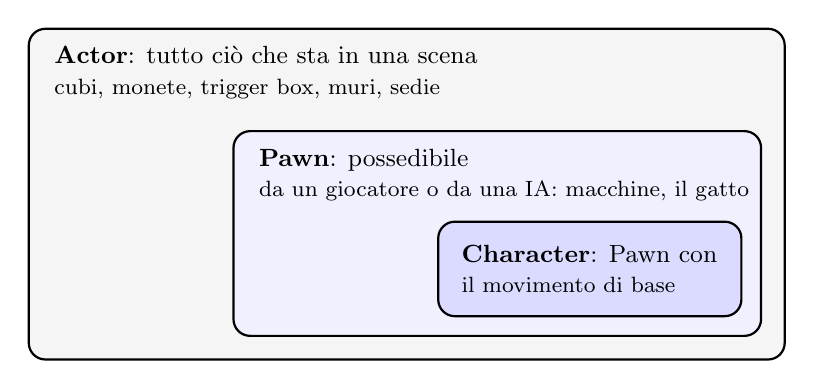
\begin{tikzpicture}[font=\small]
  \draw[thick, rounded corners=6pt, fill=gray!8] (0,0) rectangle (9.6,4.2);
  \node[anchor=north west, align=left] at (0.2,4.1)
       {\textbf{Actor}: tutto ciò che sta in una scena\\
        {\footnotesize cubi, monete, trigger box, muri, sedie}};
  \draw[thick, rounded corners=6pt, fill=blue!6] (2.6,0.3) rectangle (9.3,2.9);
  \node[anchor=north west, align=left] at (2.8,2.8)
       {\textbf{Pawn}: possedibile\\
        {\footnotesize da un giocatore o da una IA: macchine, il gatto}};
  \draw[thick, rounded corners=6pt, fill=blue!14] (5.2,0.55) rectangle (9.05,1.75);
  \node[align=left] at (7.12,1.15)
       {\textbf{Character}: Pawn con\\{\footnotesize il movimento di base}};
\end{tikzpicture}
\caption{Actor, Pawn e Character: ogni insieme è contenuto nel precedente. Un
Character è anche un Pawn, e un Pawn è anche un Actor.}
\label{gd7:fig:classi}
\end{figure}

\paragraph{Approfondimento: corpo e cervello.} Il capitolo~\ref{ue2:cap:blueprint}
(sezione~\ref{ue2:sec:classi}) riporta la gerarchia completa dal libro di
Romero e Sewell. L'immagine più utile è questa: il \textbf{Pawn} è il
\textbf{corpo}, il \textbf{Controller} che lo possiede è il \textbf{cervello}.
Un \emph{Player Controller} è il cervello di un giocatore umano, un \emph{AI
Controller} quello di un'intelligenza artificiale. Spiega anche perché, poco
prima, ruotare il personaggio era ``un pochettino più complesso'': la
rotazione della visuale passa dal Controller. E il Character porta con sé,
oltre alla mesh, una capsula per le collisioni e proprio il \textbf{Character
Movement}, che gestisce camminata, salto, nuoto e volo.

\subsection{Il Line Trace By Channel}

``Per quelli che si sentono già bravi'', un ultimo nodo, ``potentissimo'':
\textbf{Line Trace By Channel}. ``Si usa costantemente. Con questo potete fare
un FPS solo con questa cosa.'' Il docente non lo spiega: lo lascia come sfida
a chi vuole provarci, con l'invito a chiedere.

\paragraph{Approfondimento: che cosa fa un line trace.} Il nodo traccia una
\textbf{linea invisibile} tra due punti, \emph{Start} ed \emph{End}, e
restituisce il \textbf{primo oggetto colpito} lungo quella linea (con il punto
d'impatto e altre informazioni, raccolte in un \emph{Hit Result}). Il
\emph{channel} indica quale tipo di collisione considerare, per esempio
\emph{Visibility} o \emph{Camera}. Si capisce perché basti per un FPS: si
parte dalla camera, si traccia una linea nella direzione in cui si guarda, e
ciò che la linea colpisce è ciò che il proiettile ha colpito. Romero e Sewell
lo trattano nel capitolo sui \emph{trace}, insieme alla variante
\emph{Multi}, che restituisce tutti gli oggetti attraversati, e ai trace con
forme (sfere, box, capsule) invece che con una linea.

% ---------------------------------------------------------------------
\section{Le regole dei collegamenti}
\label{gd7:sec:regole}

Quando gli oggetti nell'Event Graph cominciano a essere tanti, il docente dà
due o tre ``regoline'' con cui, dice, ``fate tutto''.

\paragraph{Destra con sinistra, mai destra con destra.} Le uscite (a
\textbf{destra} di un nodo) si collegano sempre con gli ingressi (a
\textbf{sinistra} di un altro nodo). Mai destra con destra, mai sinistra con
sinistra. Non è una convenzione: ``non ha proprio senso logicamente''.
Collegare due uscite vorrebbe dire prendere un valore e, nello stesso punto,
modificarlo; ``è proprio sbagliato concettualmente''.

\paragraph{Stesso colore, stessa famiglia.} Tutte le cose dello
\textbf{stesso colore} si abbinano: se hanno lo stesso colore, probabilmente
vanno attaccate tra loro. Alcune si possono \textbf{convertire}, ma sono
poche: per esempio da intero a stringa. In quel caso ``ci pensa lui'': se le
si collega, l'editor inserisce il nodo di conversione.

\paragraph{I bianchi con i bianchi.} I pin bianchi, il flusso, si collegano
\textbf{solo con i bianchi}, e stanno \textbf{sempre in cima} al nodo: ``è
abbastanza facile''.

% ---------------------------------------------------------------------
\section{Le domande di chi parte da zero}
\label{gd7:sec:federica}

\subsection{``Che valore ha la freccina bianca?''}

Federica fa la domanda che probabilmente si stavano facendo in tanti: che
differenza c'è tra il filo bianco e quelli colorati? ``È una domanda molto
base?'' ``Normalissima, è la lezione numero uno.''

La risposta è un'immagine: bisogna pensare a delle \textbf{prese della
corrente}. L'evento (il tasto E, per esempio) è il \textbf{generatore di
corrente}, ``da dove parte tutto quanto''; tutti i nodi collegati con il
\textbf{cavo bianco} sono collegati alla corrente, e quando la corrente li
attraversa \textbf{si eseguono}. Gli altri fili \textbf{non portano corrente}:
portano soltanto \textbf{informazioni}, e da soli non eseguono nulla. I
colori dicono di che informazione si tratta: il verdino è un numero con la
virgola, il rosso un vero o falso, il rosa un testo, il blu un altro oggetto,
il giallo tre numeri con la virgola, ``che si usano solitamente per la
posizione, quindi $x$, $y$, $z$, o per la scala, quando ingrandisci
qualcosa'' (tabella~\ref{gd7:tab:tipi}). Federica: ``non avendo il programma
sotto, non avevo collegato le variabili a quei colori''.

\subsection{La corrente che fa il giro: il Delay}

Per far vedere il flusso, il docente costruisce una piccola catena sul Begin
Play. In generale la corrente, in tutti i nodi, ``entra ed esce
contemporaneamente'': entra, esce, entra, esce, \textbf{nello stesso
\emph{frame}}. ``Passa tutto uno dopo l'altro, ma assieme.'' Con un
\textbf{Delay}, invece, la corrente entra, \textbf{aspetta} (per esempio tre
secondi) e solo poi esce, facendo avvenire le cose dopo. Begin Play, Delay di
tre secondi, un'azione, un altro Delay di tre secondi, l'azione inversa: ``così
vedi proprio la corrente che fa il giro'', avanti e indietro.

\paragraph{E senza il Delay?} ``Parte subito.'' Il docente lo mostra sul
personaggio: un teletrasporto altissimo (un milione di unità sulla $z$) sul
Begin Play. Senza Delay, appena si preme Play il personaggio è già lassù. Con
un Delay di 5 secondi in mezzo, il gioco parte normalmente e dopo cinque
secondi ``finisco lassù''. Federica pensava che il Delay fosse ``una meccanica
di default che si doveva sempre fare'': ``No, no. Anzi, la maggior parte delle
cose non hanno Delay dentro.'' Serviva solo a mostrare come si controlla il
flusso del filo bianco, ``perché alla fine è sempre quello''.

\subsection{L'interfaccia, ridotta all'osso}

Le variabili, Federica le conosce già un po', per aver ``smanettato'' con
\textbf{RPG Maker}: ``non è la stessa cosa'', ma le variabili sono comuni a
tutti i linguaggi immaginabili, ``quindi vai tranquilla, è la stessa roba''.
Il suo problema è l'interfaccia nuova.

La risposta del docente è uno screenshot dell'editor su cui cancella, pezzo
per pezzo, tutto ciò che non serve: ``tutta questa parte qua sopra, bruciala
via'', i pannelli laterali via, le barre via. ``Questa è la quantità di
interfaccia che ti serve per adesso. È già un pochettino più facile.'' Nella
viewport, per ora, si tratta solo di premere Play e trascinare le cose dentro;
le parti laterali si vedranno con il corso di \textbf{level design}.

\paragraph{Come Blender.} Federica ha un po' di pratica con
\textbf{Blender}, e il docente ne approfitta: ``ti troverai super bene'',
prima di tutto con i \textbf{materiali}, che in Unreal sono schematici come in
Blender, con i nodi, come i materiali procedurali. Ma anche il codice dei
Blueprint ``è tipo Blender con i nodi, se vuoi vederla così: lo stesso
concetto''. Con un vantaggio: sono blocchetti colorati, non bisogna ricordarsi
come si scrivono le cose. ``Mi sono dimenticato una virgola?'' Non succede: si
fa tasto destro e si cerca.

\subsection{Interrompere è un favore a tutti}

Federica si scusa di far perdere tempo: ``io so che ci metto un bel po' a
capire''. La risposta merita di essere riportata per intero nel suo senso:
``fidati, è molto più importante il fatto che tu lo impari, perché sennò poi
diventa molto più grave dopo''. Anche se fra sei mesi non ci si ricorda che
cos'è il Begin Play visto oggi, ``è normalissimo''; l'unica cosa è fare
pratica. ``Siamo tutti quanti qua da due ore e 43, non da mesi.'' E soprattutto:
``quello che non hai capito tu è probabilissimo che non l'abbia capito qualcun
altro. Quindi stai aiutando qualcun altro, sicuramente.''

\subsection{Il task, riassunto}

Infine, ``l'ultima cosa, poi torno nel silenzio'': qual era il task? Il
docente lo riassume (sezione~\ref{gd7:sec:task}): \textbf{due livelli
separati} (File, New Level, Basic; qualcosa in scena; salva come
\emph{Mappa2}), uno che \textbf{porta all'altro} con un'area o una condizione
(``prendo tot monete''), e \textbf{almeno una zona} che cambia qualcosa del
personaggio: più grande, lanciato in aria, lentissimo, salto più alto, poca
frizione come sul ghiaccio. Per aprire l'altro livello, Open Level (by Object
Reference) con \emph{Mappa2} selezionata; per far ripartire quello corrente,
Open Level sullo stesso livello.

% ---------------------------------------------------------------------
\section{I progetti, e la chiusura}
\label{gd7:sec:chiusura}

Negli ultimi dieci minuti il docente chiede chi vuole mostrare il proprio
progettino su Discord. Uno studente condivide il suo: un'area che ruota il
personaggio in automatico, monete da raccogliere che teletrasportano
all'altro livello, e una zona in cui si va avanti diventando \textbf{sempre
più veloci}, ``contentissimo perché sei veloce'', finché non si sbatte contro
qualcosa e si muore. ``Progetto magnifico.'' Gli altri non si fanno avanti
(``che tristezza'').

\paragraph{Un oggetto che non deve bloccare.} Un'ultima domanda tecnica: come
fare in modo che il personaggio passi \emph{attraverso} un oggetto? Bisogna
togliergli la collisione: selezionare la mesh, scorrere fino a
\textbf{Collision} e, al posto di \emph{BlockAll}, scegliere un preset che non
blocca (per esempio \emph{OverlapAll} o \emph{NoCollision}).

\paragraph{I saluti.} ``Spero di non avervi terrorizzato con questa prima
lezione.'' L'importante è non perdersi, ``e soprattutto, se vi perdete, non
adesso''. La lezione registrata si può rivedere velocemente, ``tanto potete
skippare tre quarti di lezione'', i tratti in cui il docente gira tra i
banchi. Per dubbi e domande c'è Discord, e se è grave si può chiedere una
chiamata. Ci si rivede alla lezione successiva.\footnote{La trascrizione
riporta un'incertezza del docente sulla data (``mi sa venerdì prossimo, se non
erro\dots{} no, lunedì''); non è possibile ricostruirla con sicurezza.}

% ---------------------------------------------------------------------
\section*{Punti chiave del capitolo}
\addcontentsline{toc}{section}{Punti chiave del capitolo}

\begin{itemize}
  \item Unreal si programma in \textbf{C++} (non nel corso) o con i
        \textbf{Blueprint}, blocchetti colorati da comporre. I Blueprint si
        reggono su tre concetti: i \textbf{nodi} (tutto ciò che si può fare),
        le \textbf{variabili} (le cose che cambiano), gli \textbf{eventi}
        (l'inizio del codice).
  \item Un Blueprint ha una \textbf{viewport} (la parte visiva) e un
        \textbf{Event Graph} (il codice). Un Blueprint Class di tipo
        \textbf{Actor} è un oggetto qualsiasi; trascinato più volte nella
        scena, ogni copia esegue il proprio codice.
  \item \textbf{Begin Play} scatta quando l'oggetto viene creato,
        \textbf{Event Tick} a ogni \emph{frame}. Il \textbf{Print String}
        stampa a schermo ed è il primo strumento di debug.
  \item Tipi di variabile e colori: \textbf{Boolean} (rosso), \textbf{Integer}
        (verde acqua), \textbf{Float} (verde), \textbf{String} (rosa),
        \textbf{Vector} (giallo, tre float), riferimenti a oggetti (blu). Il
        \textbf{GET} legge, il \textbf{SET} imposta; GET + 1 + SET è il
        contatore. Compilare dopo aver creato una variabile.
  \item Sul personaggio: eventi da tastiera, \textbf{Launch Character},
        \textbf{Set Actor Scale 3D}, \textbf{Set Actor Location}; scale,
        location e rotation. Il movimento sta nel \textbf{Character
        Movement} (Jump Z Velocity, Max Walk Speed in cm/s); Pressed e
        Released fanno uno sprint.
  \item La \textbf{trigger box} è un Actor con una \textbf{Box Collision} e
        l'evento \textbf{On Component Begin Overlap}; da \textbf{Other Actor}
        si fa \textbf{Cast To ThirdPersonCharacter} per reagire solo al
        giocatore. Il \textbf{Target} di base è \emph{self}: va collegato il
        riferimento del personaggio. End Overlap per gli effetti limitati a
        un'area.
  \item \textbf{Spawn Actor} (con la transform divisa), \textbf{Destroy
        Actor}, \textbf{Simulate Physics}. Ogni componente ha parametri che
        si possono leggere e scrivere.
  \item Le \textbf{monete}: Sphere Collision + cilindro, cast, GET/+1/SET
        della variabile \textbf{sul personaggio}, Destroy Actor. Se non
        funziona, Print String per trovare dove si ferma il flusso e
        controllare le collisioni del componente giusto.
  \item Editor in \textbf{inglese} (Editor Preferences, Region \& Language);
        \textbf{Ctrl + Shift + S} come riflesso; layout recuperabile da
        Window, Load Layout.
  \item Altri nodi: \textbf{Open Level} (riaprire lo stesso livello lo
        resetta), Play Sound 2D, Quit Game, confronti + \textbf{Branch},
        \textbf{Flip Flop}, \textbf{Sequence}, \textbf{Delay}.
  \item Task in classe: \textbf{due livelli} collegati e \textbf{almeno una
        zona} che cambia un parametro del personaggio. I task avranno sempre
        requisiti minimi e tanto spazio per il resto; dal terzo-quarto task,
        codice in inglese.
  \item Tutto ciò che si muove nel tempo sull'Event Tick va
        \textbf{moltiplicato per i delta seconds}, altrimenti dipende dagli
        fps; $1/\Delta t$ è il frame rate, velocità $\times \Delta t$ dà unità
        al secondo.
  \item Le variabili \textbf{si azzerano} cambiando livello (la soluzione
        è la Game Instance). Un sistema di vita parte da un valore iniziale
        sensato e si controlla con un Branch.
  \item \textbf{Actor} (tutto), \textbf{Pawn} (possedibile),
        \textbf{Character} (Pawn con movimento). \textbf{Line Trace By
        Channel}: una linea invisibile che restituisce il primo oggetto
        colpito, la base di un FPS.
  \item Regole: uscite (destra) con ingressi (sinistra); stesso colore con
        stesso colore; il \textbf{bianco} è il flusso, la ``corrente'', e si
        collega solo con il bianco; gli altri fili sono informazioni.
        Interrompere con una domanda aiuta tutta la classe.
\end{itemize}
